\documentclass[twoside]{article}
\usepackage{amssymb}
\usepackage{amsthm}
\usepackage{amsmath}
\usepackage{amsfonts}
\usepackage[utf8]{inputenc}
\usepackage[spanish]{babel}
\usepackage{tikz}
\usepackage{centernot}
\usepackage{hyperref}
\usepackage{fancyhdr}
\usepackage{lipsum}
\usepackage{subcaption}
\hypersetup{
    colorlinks,
    citecolor=black,
    filecolor=black,
    linkcolor=black,
    urlcolor=black
}
\usepackage{xurl}
\usepackage[top=1in, bottom=1.5in, left=1in, right=1in]{geometry}
\pagestyle{fancy}
\fancyhead{}
\fancyhead[L]{\leftmark}
\fancyfoot{}
\fancyfoot[C]{\thepage}
\newcommand{\enquote}[1]{``#1''}
\usepackage{float}
\usepackage[parfill]{parskip}
\newcommand{\image}[2]{
\begin{figure}[H]
    \includegraphics[width=#1 cm]{../images/#2.png}
    \centering
\end{figure}
}

\title{Práctica 1 SWAP}
\author{XuSheng Zheng}
\date{}

\begin{document}

\maketitle
\tableofcontents
\newpage
\section{Instalación de máquinas virtuales}
Comenzamos con la instalación de las máquinas virtuales. Puesto que vamos a hacer lo mismo en ambas máquinas, vamos a centrarnos en la configuración de una de ellas:
\image{8}{1}
Le damos 4GB de RAM y 10 GB de disco duro:
\begin{figure}[H]
    \centering
    \begin{subfigure}{.5\textwidth}
        \centering
        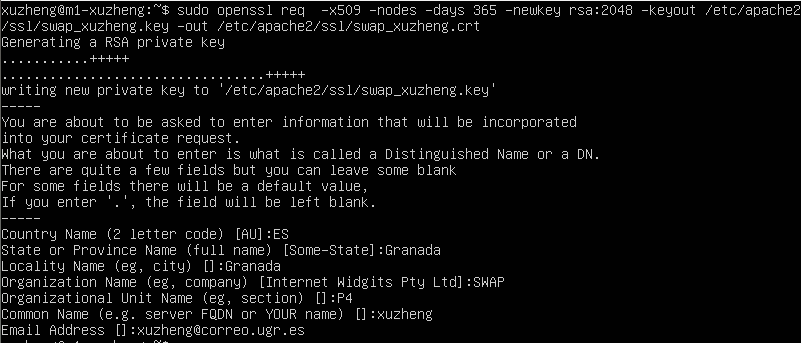
\includegraphics[width=7cm]{../images/2.png}
    \end{subfigure}%
    \begin{subfigure}{.5\textwidth}
        \centering
        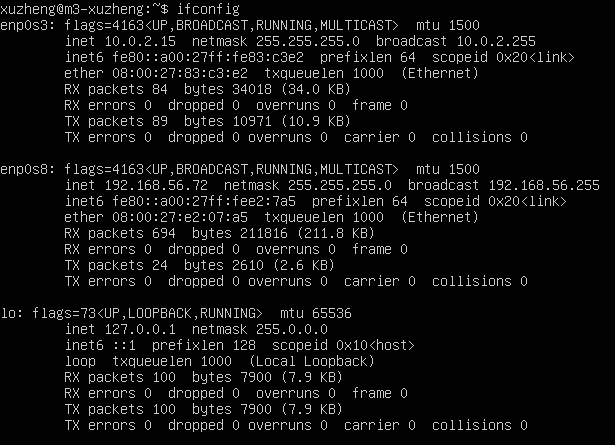
\includegraphics[width=7cm]{../images/3.png}
    \end{subfigure}
\end{figure}
Vamos a instalar Ubuntu Server, en este caso, será la 20.04:
\image{8}{4}
Arrancamos e introducimos nuestros datos dejando que nos instale SSH:
\begin{figure}[H]
    \centering
    \begin{subfigure}{.5\textwidth}
        \centering
        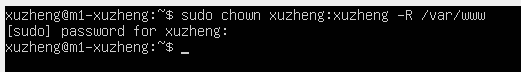
\includegraphics[width=7cm]{../images/5.png}
    \end{subfigure}%
    \begin{subfigure}{.5\textwidth}
        \centering
        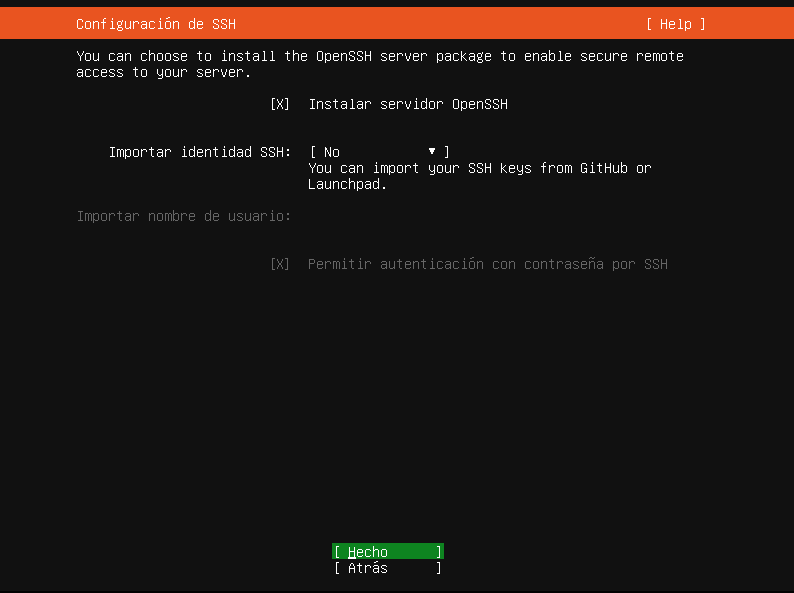
\includegraphics[width=7cm]{../images/6.png}
    \end{subfigure}
\end{figure}
\section{Configuración de red}
Una vez instalado la máquina virtual, vamos a configurar la red para permitir la conexión con Internet y con el anfitrión. En primer lugar activamos los adaptadores NAT y solo-anfitrión:
\begin{figure}[H]
    \centering
    \begin{subfigure}{.5\textwidth}
        \centering
        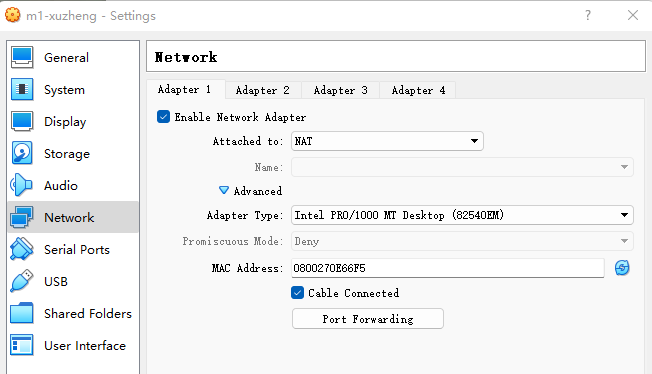
\includegraphics[width=7cm]{../images/11.png}
    \end{subfigure}%
    \begin{subfigure}{.5\textwidth}
        \centering
        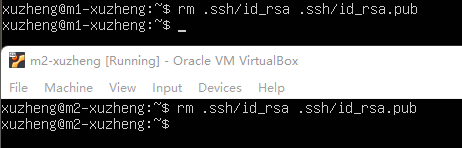
\includegraphics[width=7cm]{../images/12.png}
    \end{subfigure}
\end{figure}
Podemos usar el comando \textbf{ipconfig} en el anfitrión para ver la puerta de enlace (esta red ya estaba creada anteriormente por las prácticas de ISE):
\image{8}{13}
\subsection{Configuración de adaptadores mediante netplan}
Configuramos la red con \textbf{netplan} editando el archivo \textit{/etc/netplan/config.yaml}:
\image{8}{14}
Dejamos una interfaz que se configura mediante DHCP y otra con IP estática \textbf{192.168.56.70}. Aplicamos los cambios con \textbf{netplan apply} y comprobamos con \textbf{ifconfig}:
\image{8}{15}
\section{Instalación y configuración de Apache+PHP+MySQL}
Sigamos con la configuración de la máquina virtual instalando Apache, PHP y MySQL:
\image{10}{7}
Una vez finalizada la instalación comprobamos:
\image{10}{8}
Podemos ver que el servidor está inactivo, lo activamos:
\image{10}{9}
De mismo modo con MySQL:
\image{10}{10}
Para comprobar el funcionamiento de Apache creamos el archivo \textit{swap.html} en el directorio \textit{/var/www/\\html/}:
\image{8}{16}
En la versión de Ubuntu Server instalado, \textbf{cURL} ya está instalado de por defecto, podemos utilizarlo para acceder al archivo html creado anteriormente:
\image{8}{17}
También es posible acceder desde el anfitrión:
\image{10}{18}
\subsection{Cambio de puerto}
Para cambiar el puerto del servidor Apache modificamos los archivos \textit{/etc/apache2/ports.conf} y \textit{/etc/apache2\\/sites-enabled/000-default.conf}, en este caso, cambiamos de $80$ a $8080$:
\begin{figure}[H]
    \centering
    \begin{subfigure}{.5\textwidth}
        \centering
        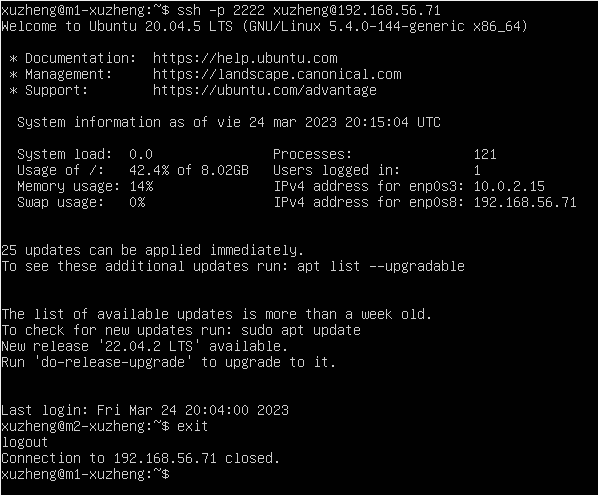
\includegraphics[width=7cm]{../images/19.png}
    \end{subfigure}%
    \begin{subfigure}{.5\textwidth}
        \centering
        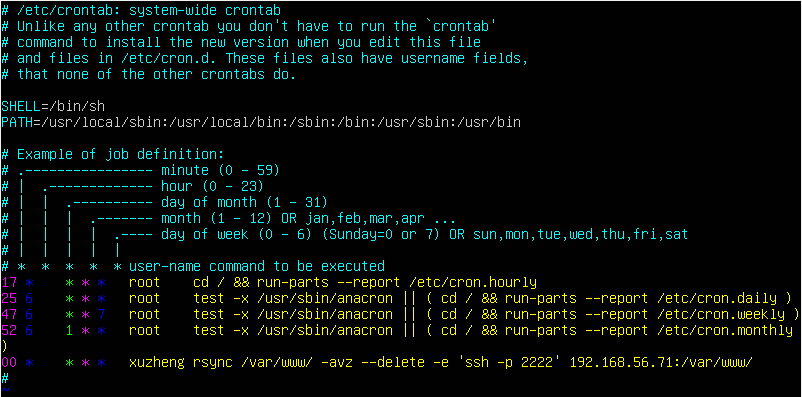
\includegraphics[width=7cm]{../images/20.png}
    \end{subfigure}
\end{figure}
Reiniciamos el servicio de Apache y comprobamos:
\image{8}{21}
\subsection{Directorio virtual}
Comenzamos creando un directorio \textit{/var/www/ejemplo/public\textunderscore html} y un archivo \textit{index.html} sencillo:
\image{6}{22}
Para evitar problemas de privilegios, ejecutamos \textbf{sudo chown -R www-data: /var/www/ejemplo}.
Ahora necesitamos crear el archivo de configuración \textit{/etc/apache2/sites-available/ejemplo.conf} como sigue:
\image{8}{23}
Activamos el directorio virtual con \textbf{sudo a2ensite ejemplo}, volvemos a habilitar el puerto $80$ en \textit{/etc/\\apache2/ports.conf} y reiniciamos Apache. Para comprobar podemos acceder desde el anfitrión:
\image{6}{24}
\subsection{Redirección de puertos}
Vamos redirigir el puerto $80$ del directorio virtual al puerto $8080$, para ello añadimos a \textit{/etc/apache2/sites-available/ejemplo.conf} las siguientes líneas: 
\image{6}{25}
Además, tenemos que ejecutar \textbf{sudo a2enmod proxy \&\& sudo a2enmod proxy\textunderscore http} para activar módulos necesarios y reiniciamos Apache. Para comprobarlo, accedemos desde el anfitrión:
\image{6}{26}
\section{Instalación y configuración de cURL}
Como habíamos mencionado anteriormente, \textbf{cURL} ya está instalado. Podemos comprobarlo con \textbf{curl \textendash\textendash version}:
\image{8}{27}
Podemos usarlo con argumento \textbf{-o} indicando el nombre del archivo que deseamos que se guarde o con argumento \textbf{-O} para descargar con el nombre original:
\image{8}{28}
\subsection{Peticiones Get/Post}
Por defecto, las peticiones que realizan \textbf{cURL} son de tipo GET, pero podemos usar cualquier método de petición mediante el argumento \textbf{-X} indicando el tipo. Como ejemplo vamos a realizar una petición POST al correo institucional:
\image{8}{29}
\subsection{Cookies}
\textbf{cURL} permite descargar cookies de sitios web mediante el argumento \textbf{-c}. También permite el envío de los mismos mediante el argumento \textbf{-b}:
\begin{figure}[H]
    \centering
    \begin{subfigure}{.5\textwidth}
        \centering
        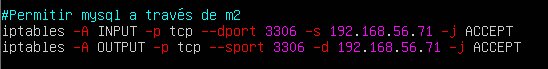
\includegraphics[width=7cm]{../images/30.png}
    \end{subfigure}%
    \begin{subfigure}{.5\textwidth}
        \centering
        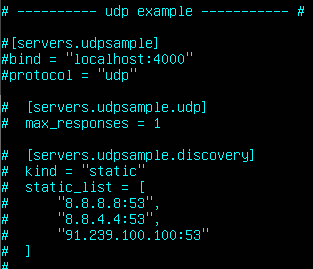
\includegraphics[width=7cm]{../images/31.png}
    \end{subfigure}
\end{figure}
\section{Configuración de SSH}
Recordemos que ya habíamos instalado SSH, para ver que funciona correctamente vamos a intentar conectar ambas máquinas:
\begin{figure}[H]
    \centering
    \begin{subfigure}{.5\textwidth}
        \centering
        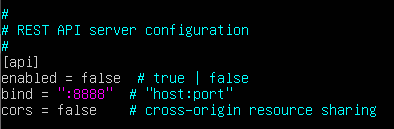
\includegraphics[width=7cm]{../images/32.png}
    \end{subfigure}%
    \begin{subfigure}{.5\textwidth}
        \centering
        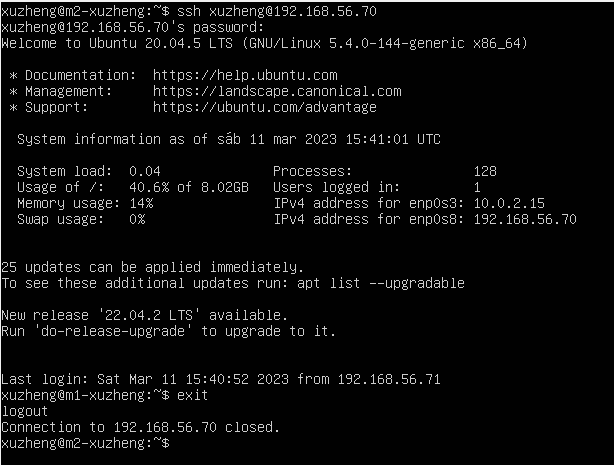
\includegraphics[width=7cm]{../images/33.png}
    \end{subfigure}
\end{figure}
\subsection{Cambio de puerto}
Para cambiar el puerto donde se conecta SSH, necesitamos configurar el archivo \textit{/etc/ssh/sshd\textunderscore config}. En este caso, usaremos el puerto $2222$ en ambas máquinas:
\image{8}{34}
Después de guardar los cambios tenemos que reiniciar el servicio SSH. Una vez reiniciado, para conectarnos hace falta especificar el puerto mediante el argumento \textbf{-p}:
\image{8}{35}
\subsection{Conexión sin contraseña}
En primer lugar, necesitamos generar el par de claves pública y privada. Lo hacemos con el comando \textbf{ssh-keygen} dejando los campos vacíos como sigue:
\image{8}{36}
Una vez creadas en ambas máquinas copiamos la clave pública a la máquina contraria:
\begin{figure}[H]
    \centering
    \begin{subfigure}{.5\textwidth}
        \centering
        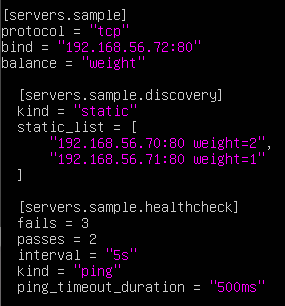
\includegraphics[width=7cm]{../images/37.png}
    \end{subfigure}%
    \begin{subfigure}{.5\textwidth}
        \centering
        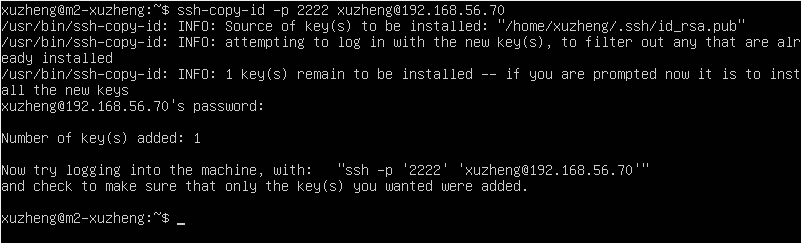
\includegraphics[width=7cm]{../images/38.png}
    \end{subfigure}
\end{figure}
Ahora al intentar conectar ya no nos pide la contraseña:
\begin{figure}[H]
    \centering
    \begin{subfigure}{.5\textwidth}
        \centering
        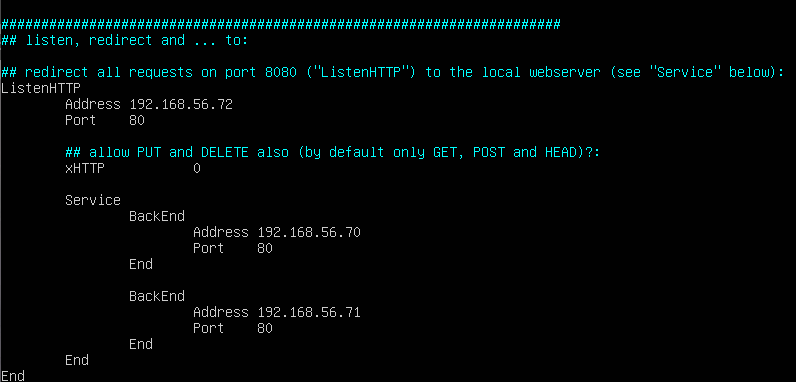
\includegraphics[width=7cm]{../images/39.png}
    \end{subfigure}%
    \begin{subfigure}{.5\textwidth}
        \centering
        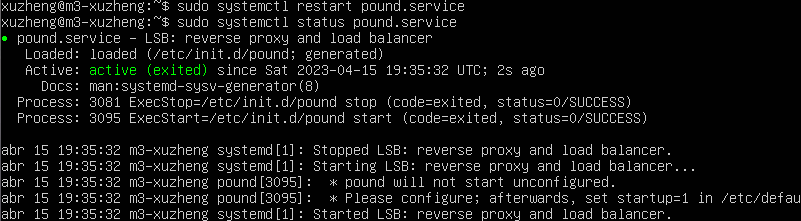
\includegraphics[width=7cm]{../images/40.png}
    \end{subfigure}
\end{figure}
\newpage
\section{Bibliografía}
\begin{itemize}
    \item \url{https://ubiq.co/tech-blog/how-to-change-port-number-in-apache-in-ubuntu/}
    \item \url{https://elpuig.xeill.net/Members/vcarceler/articulos/configuracion-basica-en-ubuntu-20-04-server}
    \item \url{https://linuxize.com/post/how-to-set-up-apache-virtual-hosts-on-ubuntu-18-04/?utm_content=cmp-true}
    \item \url{https://reqbin.com/req/c-g5d14cew/curl-post-example}
    \item \url{https://curl.se/docs/manpage.html}
    \item \url{https://www.ionos.com/help/server-cloud-infrastructure/getting-started/important-security-information-for-your-server/changing-the-default-ssh-port/}
    \item \url{https://www.ibm.com/support/pages/configuring-ssh-login-without-password}
\end{itemize}

\end{document}
